%%%%%%%%%%%%%%%%%%%%%%%%%%%%%%%%%%%%%%%%%%%%%%%%%%%%%%%%%%%%%%
%%%%
%%%%  Project October
%%%%
%%%%%%%%%%%%%%%%%%%%%%%%%%%%%%%%%%%%%%%%%%%%%%%%%%%%%%%%%%%%%%
\documentclass[11pt,letterpaper]{article}
\usepackage[utf8]{inputenc}
\usepackage[letterpaper,includeheadfoot, top=0.5cm, bottom=3.0cm, right=2.0cm, left=2.0cm]{geometry}
\renewcommand{\familydefault}{\sfdefault}

\usepackage{graphicx}
\usepackage{color}
\usepackage{amsmath}
\usepackage{fancyhdr}
\usepackage{hyperref}
\usepackage{subfig}
\usepackage{pdfpages}
\usepackage{amssymb}
\usepackage{url}
\usepackage{listings}

\usepackage{listings} %Code
\lstset{language=C, tabsize=4,framexleftmargin=5mm,breaklines=true}

\begin{document}
%\begin{sf}

\newpage
\pagestyle{fancy}
\fancyhf{}
\fancyhead[L]{ 
\includegraphics[scale=0.3]{img/cwru-formal-logo-blue-no-tag.png} }
\vspace*{6cm}
\begin{center}
\Huge  {Project October}\\
\vspace{1cm}
\huge {Read news that you want to read}\\
\vspace{1cm}
\end{center}
%----------------- Names ------------------------
\vfill
\begin{flushright}
\begin{tabular}{ll}
Authors: & Rajesh Cherukuri, Tom Dooner, Mika Little, Brian Stack\\
Project: & Project October\\
Date: & \today
\end{tabular}
\end{flushright}

\newpage
\pagestyle{fancy}
\fancyhf{}

%\fancyhead[L]{\rightmark}
\fancyhead[L]{\small \rm \textit{\rightmark}}
\fancyhead[R]{\small \rm \textbf{\thepage}}


%\fancyfoot[L]{\small \rm \textit{Pie de página - Izquierda}}
%\fancyfoot[R]{\small \rm \textit{Pie de página - Derecha}}
%\fancyfoot[C]{\thepage} %Centro

\renewcommand{\sectionmark}[1]{\markright{\thesection.\ #1}}
\renewcommand{\headrulewidth}{0.5pt}
\renewcommand{\footrulewidth}{0.5pt}

% =============== Index ===============

\tableofcontents
\listoffigures

% =============== Section ===============
\newpage
\section{Abstract}

In modern news aggregation services, such as Reddit, Slashdot, Digg, and Hacker News, longtime members report noticing a marked decrease in quality of discourse as the services gain mainstream attention.
This gradual but irreversible decline caused by the influx of new users dates back to the newsgroup era, when new college students would log in for the first times in September.
After AOL opened newsgroups to the masses, the community standards continued to devolve, according to newsgroup veterans\cite{september}.

The inevitable loss of the longtime members further perpetuates the problem, and causes large numbers of excellent contributors to feel out-of-place in their own community.
We aim to engineer a service that uses technological principles to avoid this, thus improving the user experience and allowing a large community to benefit from thoughtful discourse and interesting articles. \\

\newpage

%----Everything else----%

\section{Project October: Hybrid Recommender System}

Due to the enormous amount of information available online, the need for a highly developed personalization and filtering system is growing permanently.
Recommender systems constitute a specific type of information filtering that attempt to present items according the interests expressed by a user\cite{1}.
Most web recommenders are employed for e-commerce applications or customer adapted websites, which assist users in decision making by providing personalized information \cite{5}, but the same techniques that suggest related items on e-commerce websites can recommend news articles to users who will enjoy reading them.
We believe Project October is the first attempt to apply recommendation techniques to social news aggregation.

\subsection{Background}
It is our hypothesis that recommendation of news sources will provide a scalable community experience that can be tailored to each person's interests.
Providing an automatic, customized, recommendation of articles will prevent the community from being diluted by new users thus preventing the Eternal September phenomenon.
Users that prefer intellectual discourse will automatically be recommended articles and comments that fit such a criteria, and users that prefer simpler entertainment will be recommended such stories.

This proposal discusses an implementation of a hybrid collaborative and content-based filtering approach for a web-based recommender system (``October'').
In particular, we will be linking various news sources and user submitted sources.
The resulting network of user-item relations and associated content features is converted into a unified mathematical model, which is applicable to our underlying neighbor-based prediction algorithm.
By means of various experiments, we demonstrate the influence of supplementary users as well as item features on the prediction accuracy of October, our proposed hybrid recommender. In order to decrease system runtime and to reveal latent user and item relations, we factorize our hybrid model via singular value decomposition (SVD).

For the development and evaluation of our proposed hybrid recommender system, we make use of various news outlets and user recommendations, importing them into a graph database.
Both corpora are joined in a unified mathematical model, which describes the complex network of interdependencies.

\subsection{Intended Audience}
% The audience is power web users that want the most accurate news source possible
\subsection{Requirements}
\subsubsection{Frontend}
The frontend will be a standard social news aggregator, similar to Reddit or Hacker News.
Upon going to the homepage, logged-out users will be presented with a splash page that describes the allure of Project October and offers a registration link.
Users can register for the application by selecting a username and password.

When logged in, users will be presented with their personalized content.
We are modeling the design after the front page of a newspaper -- articles that we judge to be more interesting to a user will be placed in the most prominent positioning, and articles that are less important will fill the side columns and occupy less space.
Users will be able to click on the headline (or associated image, if existent) to be taken to the original news source.

Each news article will feature a link to view the associated comments and it will feature a corner icon of how much credibility (``cred'') a given article possesses.
This is analogous to upvoting in Reddit, except that giving an article cred on October will inform the recommendation engine of your individual preference, rather than directly impacting the weighting of an article by a predefined formula.

\subsubsection{Backend}
% The backend will use a graph database, yadda yadda

\subsubsection{Frontend/Backend API}
October will employ an API to promote separation between the frontend and the backend recommender system.
This will provide a clear interface and facilitate easy simultaneous development of both parts of October.

To implement the API, we will use Apache Thrift, an Interface Description Language originally developed by Facebook\cite{thrift}.
The essence of the API is simple, featuring primarily two types of calls:
\begin{description}
\item[Give recommendations for user $n$]
This is the main output from the backend, returning recommended news stories or comments for a given user.
Ancillary parameters will be added to this to facilitate the frontend placement of articles, e.g. the recommendation confidence and individual article weightings.
\item[User took action $n$]
This is the main input to the backend, allowing it to adjust recommendations according to user action.
The parameters to this API call can be of many types. For example, "User commented on article \#$n$", "User gave cred to comment \#$n$", and "User visited link \#$n$" are all valid parameters for this API call.
\end{description}

\subsection{Project Management}
We will manage the project using agile development strategies.

\subsubsection{Agile Development}
In order to schedule work, we have employed Pivotal Tracker, an online task management solution.
From the queue, we will assign tasks as we finish previous tasks.
The work naturally fits into two main categories -- frontend and backend.
Work relating to each category will be assigned to the same people until we make enough progress to cross between teams at will.
At least until that point, Brian and Rajesh will work on the backend while Tom and Mika create the frontend.

\subsubsection{Scrum}
We will meet every Monday, Wednesday, and Friday at 3:55pm to have a short meeting to discuss the current progress.

\subsubsection{Iterations}
% We will have iterations of one week in duration
% Perhaps discuss the actual plans for the next few iterations?






%As mentioned earlier, the prediction accuracy of our developed hybrid recommender depends on several different parameters, like neighborhood size, data dimension, utilized features and so on. This section will investigate the behavior of our system under certain conditions. We will be using the well known Root Mean Squared Error (metric used in the Netflix Prize Competition): $RMSE(O,P) = \sqrt{\frac{\sum_{i=1}^{n} (O_{i} - P_{i})^{2}}{n}}$ (where $O$ and $P$ are vectors of observed and predicted values respectively). RMSE will compute how close the estimates are to the values actually observed.\\

%Finally, we are going to compare the overall performance of October with other implementation variants, at which prediction accuracy as well as computational effort are scrutinized.

% \subsubsection{Neighborhood Size}

%In general there exist two basic implementation variants of the KNN-algorithm, namely user- and item-oriented collaborative filtering. Whereas user-oriented techniques just consider like-minded users to predict unknown ratings, item-oriented methods utilize similar items \cite{10,13}. However both collaborative filtering variants employ the same underlying mathematical approach, in which the current examined user/item rating is estimated based on the $k$-nearest neighbors.

%Obviously our item-oriented approach performs much better than the user-oriented implementation, which agrees with the general observations about collaborative filtering systems that can be found in most literature \cite{8, 2}, and might be explained by the fact that individuals are more familiar with the items previously preferred than with potential like-minded users.

%The comparison furthermore reveals that a relatively small neighborhood produces imprecise rating estimates, which is due to the fact that the considered users or rather items do not contain sufficient information to make reliable predictions. However, in case of a comparatively large neighborhood it might happen that too many users or items with very low similarities are taken into account \cite{4, 6}.

%For our further analysis we will make use of the optimum neighborhood size determined for user-oriented and item-oriented collaborative filtering respectively ($n = 25/70$).

% \subsubsection{Data Dimension}

%The prediction accuracy of our hybrid recommender system furthermore depends on the dimension k of the decomposed matrices (V, S and W; see Eq.(5)) \cite{10, 4}. Whereas relatively short singular vectors do not have enough explanatory power to differentiate the appropriate users or items, comparatively long vectors might lead to over-fitting.\\

%As before, the item-oriented implementation produces better prediction results than the user-oriented counterpart. The displayed mixed approach of our SVD-KNN algorithm can be described as a weighted combination ($70$/$30$ ratio o user/item oriented collaborative filtering estimates) of user-oriented and item-oriented prediction results. However, this method could only achieve considerable performance improvements when supplementary user or rather item features were taken into account.\\

%According to the comparison of the individual methods and the combined method, the global minimum of our user-oriented as well as mixed collaborative filtering approach is reached at a dimension of k = 10. For further studies on our item-oriented approach we set k = 20, because the dimension of the global minimum is quite high (k = 40) and produces an unsatisfactory system runtime.

% \subsubsection{Feature Weights}

%Besides analyzing the influence of neighborhood size and data dimension, we additionally investigate the effect of the retrieved user- and item-features on the prediction accuracy of our design hybrid recommender. As mentioned earlier, the contribution of the single user and item features is regulated by weights. We can show the behavior of October under the influence of various weighted features, employing the optimal parameter settings determined previously ($n = \frac{25}{70}$ and $k=\frac{10}{20}$). \\

%All user and item features are selected based on their matrix fill-rate, where as only feature matrices with a low sparsity ($\leq 99\% $) are considered for rating prediction. This is due to the fact that sparse feature matrices do not increase the explanatory power of our original rating matrix R. In our research, we investigate public user profile information of the examined Freebase users as well as geolocation, date, and category of the appropriate media.\\

%The performance improvement made by the examined media features is much higher than by the considered user features. In particular, the Media-\{Age-Country\} feature produced surpassing prediction results. But the highest prediction accuracy could be achieved by the combination of both individual user and item features. This can also be evidenced by taking the item- or user-oriented collaborative filtering methods using similar features, which still show that October outperforms them to provide lower RMSE values across the board.

%Besides contrasting the prediction accuracy of these algorithms, we furthermore want to scrutinize their runtime. We can show a juxtaposition of the individual rating prediction methods, where the computational effort is presented on a logarithmic scale. Note that the algorithm runtime is directly dependent on the available processing power.

%In general, the performance and runtime of recommender systems are in competition and have a mutual influence on each other. For this reason we need to treat a recommender with all its factors as a whole. According to performance benchmarks, our proposed hybrid recommender October is superior in terms of prediction accuracy. Although the pure SVD approach shows the lowest computational effort, our hybrid method is about four times faster than traditional KNN collaborative filtering. On that account we believe that October is practical to media recommendation for real-world users.

% \subsection{Algorithm}

% ---To be added--------------------

% ----------------------------------



% ============= References ==============
\newpage
\newpage
\begin{thebibliography}{13}
  \bibitem{1} Gediminas Adomavicius , Alexander Tuzhilin, \textit{Toward the Next Generation of Recommender Systems: A Survey of the State-of-the-Art and Possible Extensions}, IEEE Transactions on Knowledge and Data Engineering, v.17 n.6, p.734-749, June 2005  [doi>10.1109/TKDE.2005.99]

  %\bibitem{2} Robert M. Bell , Yehuda Koren, \textit{Scalable Collaborative Filtering with Jointly Derived Neighborhood Interpolation Weights, Proceedings of the 2007 Seventh IEEE International Conference on Data Mining}, p.43-52, October 28-31, 2007  [doi>10.1109/ICDM.2007.90]

  %\bibitem{3} R. D. Burke. Hybrid web recommender systems. In P. Brusilovsky, A. Kobsa, and W. Nejdl, editors, \textit{The Adaptive Web, Methods and Strategies of Web Personalization}, volume 4321 of Lecture Notes in Computer Science, pages 377--408. Springer, 2007.

  %\bibitem{4} Yehuda Koren, \textit{Factorization meets the neighborhood: a multifaceted collaborative filtering model}, Proceeding of the 14th ACM SIGKDD international conference on Knowledge discovery and data mining, August 24-27, 2008, Las Vegas, Nevada, USA  [doi>10.1145/1401890.1401944]

  \bibitem{5} Greg Linden , Brent Smith , Jeremy York, \textit{Amazon.com Recommendations: Item-to-Item Collaborative Filtering}, IEEE Internet Computing, v.7 n.1, p.76-80, January 2003  [doi>10.1109/MIC.2003.1167344]

  %\bibitem{6} Prem Melville , Raymod J. Mooney , Ramadass Nagarajan, \textit{Content-boosted collaborative filtering for improved recommendations, Eighteenth national conference on Artificial intelligence}, p.187-192, July 28-August 01, 2002, Edmonton, Alberta, Canada

  %\bibitem{7} M. J. Pazzani and D. Billsus. \textit{Content-based recommendation systems}. In P. Brusilovsky, A. Kobsa, and W. Nejdl, editors, The Adaptive Web, volume 4321 of Lecture Notes in Computer Science, chapter 10, pages 325--341. Springer-Verlag, Berlin, Germany, May 2007.

  %\bibitem{8} Badrul Sarwar , George Karypis , Joseph Konstan , John Reidl, \textit{Item-based collaborative filtering recommendation algorithms}, Proceedings of the 10th international conference on World Wide Web, p.285-295, May 01-05, 2001, Hong Kong, Hong Kong  [doi>10.1145/371920.372071]

  %\bibitem{9} B. M. Sarwar, G. Karypis, J. A. Konstan, and J. T. Riedl. \textit{Application of dimensionality reduction in recommender system - a case study}. In In ACM WebKDD Workshop, 2000.

  %\bibitem{10} J. B. Schafer, D. Frankowski, J. Herlocker, and S. Sen. \textit{Collaborative filtering recommender systems}. In P. Brusilovsky, A. Kobsa, and W. Nejdl, editors, The Adaptive Web, volume 4321 of Lecture Notes in Computer Science, chapter 9, pages 291--324. Springer-Verlag, Berlin, Germany, may 2007.

  %\bibitem{11} David H. Stern , Ralf Herbrich , Thore Graepel, \textit{Matchbox: large scale online bayesian recommendations}, Proceedings of the 18th international conference on World wide web, April 20-24, 2009, Madrid, Spain  [doi>10.1145/1526709.1526725]

  %\bibitem{12} A. Toescher, M. Jahrer, and R. Legenstein. \textit{Improved neighborhood-based algorithms for large-scale recommender systems}. In KDD '08: Proceeding of the 14th ACM SIGKDD international conference on Knowledge discovery and data mining, Graz, Austria, 2008. ACM.

  %\bibitem{13} Jun Wang , Arjen P. de Vries , Marcel J. T. Reinders, \textit{Unifying user-based and item-based collaborative filtering approaches by similarity fusion}, Proceedings of the 29th annual international ACM SIGIR conference on Research and development in information retrieval, August 06-11, 2006, Seattle, Washington, USA  [doi>10.1145/1148170.1148257]

  \bibitem{september} \url{http://en.wikipedia.org/wiki/Eternal\_September}
  \bibitem{thrift} \url{http://en.wikipedia.org/wiki/Apache\_Thrift}
\end{thebibliography}

% ============= Database Schematic ==============
\begin{figure}
\centering
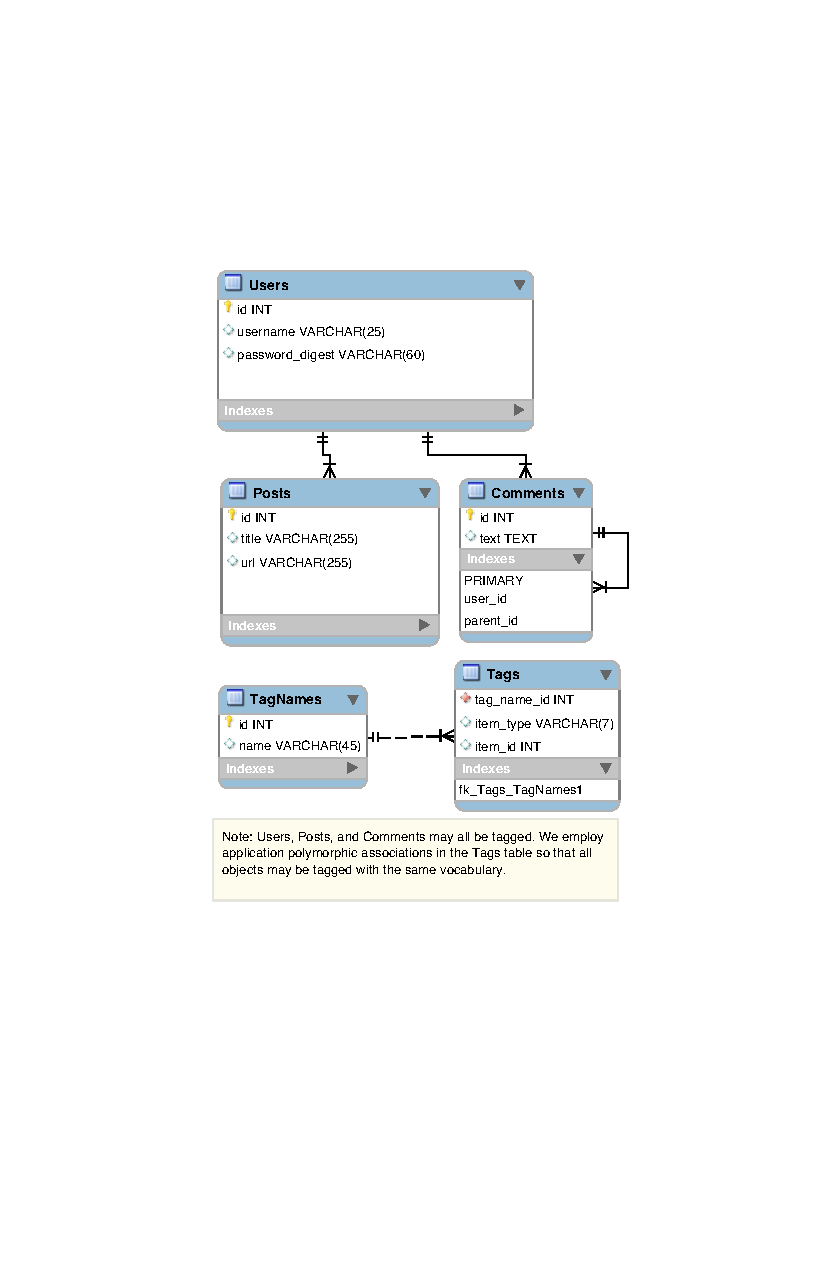
\includegraphics{db_diagram.pdf}
\caption{Frontend Database Relational Diagram}
\label{fig:database}
\end{figure}

% ============= FIN ==============

\end{document}
